% ==============================================================================
% CHAPTER 1: INTRODUCTION
% ==============================================================================
\chapter{Introduction}
\section{Overview}
Small and Medium-sized Enterprises (SMEs), particularly independent grocery stores, convenience retailers, and local distributors, represent the bedrock of the commercial supply chain in emerging and established economies alike. Unlike corporate hypermarket chains with dedicated operations research divisions and multi-million-dollar enterprise infrastructure, retail SMEs typically operate on razor-thin operating margins, often between 2\% and 5\%. Under such precarious margins, operational profitability is determined almost entirely by the precision of inventory working capital management.

In traditional retail environments, store managers are confronted with two conflicting failure modes:
\begin{enumerate}
    \item \textbf{The Overstocking Penalty:} Purchasing excessive inventory locks up critical working capital, incurs holding costs approximating 20\% to 35\% of inventory value annually, and increases losses from shrinkage, damage, and shelf-life expiration on perishable lines.
    \item \textbf{The Stockout Penalty:} Under-purchasing leads directly to lost sales revenue, backorders, and customer churn, as consumers frequently defect to competing neighborhood grocers when everyday staples are unavailable.
\end{enumerate}

Despite these substantial operational risks, modern computational inventory solutions remain largely out of reach for small retail operators. Contemporary commercial Enterprise Resource Planning (ERP) platforms---such as SAP S/4HANA, Microsoft Dynamics 365, and Oracle NetSuite---are fundamentally engineered for multinational enterprises. They mandate continuous high-speed internet connectivity, high upfront deployment costs, ongoing Software-as-a-Service (SaaS) subscription overheads, and complex manual parameterization that requires dedicated technical specialists. When independent retailers attempt to digitize, they often resort to disconnected electronic point of sale (POS) cash registers or static electronic spreadsheets. While these tools record historical transactions, they lack embedded intelligence to anticipate future demand fluctuations, analyze non-stationary seasonal sales trends, or systematically compute replenishments.

To address this technological disparity, this project presents \textbf{NexusERP}: an intelligent, lightweight, edge-first ERP management and predictive demand forecasting system designed specifically for SME retail environments. NexusERP unites an atomic local POS billing engine, an automated multi-model machine learning demand forecasting tournament, and a scientific $(s, S)$ periodic inventory replenishment pipeline into a single, cohesive, offline-capable application.

\section{Problem Statement}
Independent SME retail store managers routinely rely on manual inspection, personal recollection, or crude static min-max rules to replenish inventory. This intuitive approach leads to severe stockouts during unforeseen demand surges, alongside unnecessary capital lockup in slow-moving stock-keeping units (SKUs). 

Existing commercial ERP systems fail to serve this segment because they impose prohibitive subscription costs, depend strictly on centralized cloud availability, and lack lightweight, automated demand forecasting tailored to localized sales variance. Consequently, there exists an acute need for an offline-first, computationally lightweight ERP platform that autonomously predicts multi-horizon item demand, classifies inventory volatility without manual tuning, and translates statistical forecasts directly into automated, actionable reorder recommendations.

\section{Motivation and Objectives}
The primary motivation behind NexusERP is democratizing advanced operations research and machine learning forecasting tools for small business owners who lack data science expertise and cannot afford enterprise software subscriptions. By embedding automated algorithm selection directly into an intuitive, touch-friendly retail checkout and inventory management interface, NexusERP eliminates the barrier between predictive analytics and physical procurement.

The specific technical and operational objectives of this project are:
\begin{enumerate}
    \item \textbf{Develop an Offline-First 3-Tier ERP Architecture:} Build a decoupled, high-performance local ERP system utilizing FastAPI (Python 3.11+), React 19, and an ACID-compliant embedded SQLite database, capable of executing 100\% of operations without cloud connectivity.
    \item \textbf{Implement Mathematical Demand Pattern Classification:} Integrate the Syntetos-Boylan Classification (SBC) framework using Average Demand Interval ($ADI$) and Squared Coefficient of Variation ($CV^2$) to partition product catalogs into Regular, Erratic, Intermittent, and Lumpy quadrants.
    \item \textbf{Build an Automated Multi-Model Forecasting Tournament:} Construct an automated competition engine that trains and evaluates candidate time-series models (Facebook Prophet, Holt-Winters Exponential Smoothing, Random Forest Regressors, Gradient Boosting, and Simple Exponential Smoothing) over rolling holdout splits, dynamically selecting the minimum Mean Absolute Error (MAE) model per SKU.
    \item \textbf{Establish Scientific Periodic Replenishment Logic:} Formulate automated safety stock ($SS$) and reorder point ($ROP$) mechanisms governed by statistical service levels, providing managers with clear 7-day restocking volume recommendations.
    \item \textbf{Integrate an Atomic POS and Procurement Lifecycle:} Engineer real-time POS billing with dynamic cart validation, atomic inventory decrementing, 80mm ESC/POS thermal receipt formatting, and an end-to-end 4-stage Purchase Order (PO) workflow.
\end{enumerate}

\section{Scope and Limitations}
\subsection{Project Scope}
The scope of this project encompasses:
\begin{itemize}
    \item Full local transaction processing across Point of Sale (POS), Inventory, and Purchase Order management.
    \item Historical transaction ingestion, time-series feature engineering, and automated model competition over 30 canonical fast-moving retail SKUs.
    \item Visual dashboard analytics, including ABC-XYZ inventory segmentation and interactive forecast curve rendering.
    \item Persistent disk caching of precomputed model forecasts for sub-50-millisecond query responses on resource-constrained host hardware.
\end{itemize}

\subsection{Limitations}
\begin{itemize}
    \item \textbf{Multi-Store Distributed Synchronization:} Multi-branch database synchronization across wide-area networks is outside the current Phase I offline single-node implementation scope.
    \item \textbf{Automated Banking Electronic Data Interchange (EDI):} Financial settlement gateways and automated bank wire transfers are excluded; payments are logged at the POS cash/card ledger level.
    \item \textbf{Proprietary Hardware Drivers:} System interactions with external receipt printers rely on standard browser-mediated printing subsystems rather than direct proprietary binary device drivers.
\end{itemize}

\section{Methodology Overview}
The development methodology follows an iterative engineering lifecycle:
\begin{enumerate}
    \item \textbf{System Specification \& Requirements Gathering:} Analyzing operational SME retail workflows to define relational schemas, transactional safety constraints, and forecast latency targets.
    \item \textbf{Data Modeling \& Backend Construction:} Implementing asynchronous RESTful endpoints in FastAPI and relational mappings in SQLAlchemy 2.0 with atomic transaction boundaries.
    \item \textbf{Algorithmic Engine Development:} Developing the mathematical SBC classifier, feature extraction pipelines (lag vectors, rolling averages), and candidate model evaluation harnesses.
    \item \textbf{Frontend User Interface Construction:} Assembling a component-driven React 19 SPA utilizing Tailwind CSS tokens, Vite compilation, and Recharts SVG data visualization.
    \item \textbf{Empirical Evaluation \& Validation:} Benchmarking forecast accuracy across 54,780 daily transaction records to verify model convergence and operational throughput.
\end{enumerate}

\section{Report Organization}
The remainder of this report is organized as follows: Chapter 2 reviews literature in retail ERP and forecasting. Chapter 3 details system design, requirements, and database architecture. Chapter 4 explains the core mathematical classification and tournament methodology. Chapter 5 presents empirical results, interface walkthrough, and the Phase II roadmap.


% ==============================================================================
% CHAPTER 2: LITERATURE SURVEY
% ==============================================================================
\clearpage
\chapter{Literature Survey}
\section{Evolution of ERP Systems in Retail SMEs}
Enterprise Resource Planning (ERP) systems originated in material requirements planning (MRP) systems of the 1970s, steadily evolving into comprehensive platforms that integrate accounting, sales, inventory, and supply chain logistics into a centralized relational database. In commercial enterprise environments, suites such as SAP S/4HANA and Oracle ERP Cloud have demonstrated marked improvements in inventory visibility and operational synchronization \cite{10}. 

However, Chapman \cite{10} identified that over 65\% of conventional ERP deployments in small and medium-sized enterprises either fail to meet operational targets or run significantly over budget. The primary barriers cited include excessive architectural bloat, rigid operational workflows that conflict with informal small-business practices, and high total cost of ownership (TCO). Furthermore, contemporary cloud-hosted SaaS ERP paradigms presuppose uninterrupted high-bandwidth connectivity. In emerging suburban and rural markets where local power or internet disruptions occur, cloud-dependent cash registers fail to conduct point-of-sale transactions, halting business operations. Consequently, literature highlights the necessity of lightweight, offline-first architectures that preserve local autonomy while offering advanced analytical intelligence.

\section{Time-Series Demand Forecasting Methodologies}
Accurate demand forecasting is essential for mitigating information distortion across retail supply networks, famously formalized by Lee et al. \cite{8} as the ``bullwhip effect.'' Traditional retail inventory models predominantly employed classical statistical techniques:

\subsection{Classical Statistical Approaches}
Single Exponential Smoothing (SES) and Holt-Winters (HW) additive/multiplicative models \cite{5, 15, 16} have long formed the foundational baseline for commercial forecasting. While Holt-Winters effectively captures linear trends and regular seasonal fluctuations, Gardner \cite{5} noted that it struggles when sales exhibit non-linear regime shifts, sudden promotion-driven spikes, or extended periods of zero sales.

\subsection{Bayesian Additive and Generalized Additive Models}
To address the limitations of classical statistical approaches, Taylor and Letham \cite{2} introduced \textbf{Prophet}, an open-source decomposable time-series framework developed by Meta. Prophet models time series through a generalized additive model (GAM) formulated as:
\begin{equation}
y(t) = g(t) + s(t) + h(t) + \epsilon_t
\end{equation}
where $g(t)$ models non-periodic piecewise linear or logistic growth trends, $s(t)$ represents periodic seasonal components modeled via Fourier series, $h(t)$ incorporates irregular holiday/event effects, and $\epsilon_t$ captures normally distributed idiosyncratic errors. By handling missing data, calendar shifts, and trend changepoints robustly without requiring stationary differencing, Prophet has achieved high empirical success in commercial forecasting benchmarks \cite{9}.

\subsection{Supervised Machine Learning and Tree Ensembles}
In parallel, machine learning algorithms---notably Breiman's Random Forest \cite{12} and Friedman's Gradient Boosting Machines \cite{13}---have gained prominence for demand prediction \cite{11}. By re-framing time-series forecasting as a supervised tabular regression problem through feature engineering (e.g., historical sales lags, rolling window statistics, day-of-week cyclical encodings), ensemble tree regressors capture complex non-linear feature interactions without making strict parametric assumptions regarding error distributions. Carbonneau et al. \cite{11} demonstrated that machine learning ensembles frequently outperform classical regression models on volatile, non-linear retail time series.

\section{Intermittent Demand and Demand Classification}
A critical vulnerability in retail forecasting is the misapplication of continuous forecasting models to intermittent or slow-moving items. In retail grocery catalogs, a substantial proportion of stock-keeping units exhibit zero demand on multiple consecutive days, punctuated by sporadic customer purchases. 

Croston \cite{4} recognized that applying standard exponential smoothing to intermittent demand produces biased, mathematically inconsistent estimates immediately following non-zero transactions. Croston proposed decomposing the series into two independent components: demand size when transactions occur, and inter-arrival intervals between positive demand periods. Building upon Croston's foundation, Syntetos and Boylan \cite{1} established a formal demand classification taxonomy based on two mathematical dimensions:
\begin{enumerate}
    \item \textbf{Average Demand Interval ($ADI$):} The average duration between successive non-zero transactions.
    \item \textbf{Squared Coefficient of Variation ($CV^2$):} The normalized variance of positive transaction order sizes.
\end{enumerate}
Syntetos and Boylan demonstrated that partitioning products into four quadrants (Regular, Erratic, Intermittent, and Lumpy) allows systems to avoid catastrophic forecasting errors by dynamically selecting algorithm families appropriate to each item's physical velocity.

\section{Scientific Replenishment Policies and (s, S) Control}
Point forecasts of future demand are operationally useless unless translated into concrete procurement decisions. In classical inventory theory, Silver, Pyke, and Peterson \cite{7} formulated the continuous review $(s, Q)$ and periodic review $(s, S)$ inventory control frameworks. Under a periodic $(s, S)$ policy with review period $R$ and supplier lead time $L$, physical stock is inspected at fixed intervals. If on-hand stock falls to or below the reorder point $s$, a replenishment order is dispatched to raise total inventory position up to the target level $S$.

Chan et al. \cite{14} proved that establishing dynamic safety stock buffers proportional to forecast standard error and lead-time variance ensures target service levels (e.g., 95\% or 99\% non-stockout probability) while minimizing overall capital allocation. Furthermore, Scholz-Reiter et al. \cite{17} validated that coupling demand classification with ABC-XYZ inventory segmentation provides managers with transparent, risk-adjusted replenishment thresholds.

\section{Comparative Summary of Related Works}
Table \ref{tab:literature_survey} synthesizes key literature in retail inventory management, highlighting the distinct architectural gap bridged by NexusERP.

\begin{table}[H]
\centering
\caption[Comparative Analysis of Related Works]{Comparative Analysis of Related Works in Retail ERP and Demand Forecasting}
\label{tab:literature_survey}
\resizebox{\textwidth}{!}{%
\begin{tabular}{|p{3.2cm}|p{3.5cm}|p{3.2cm}|p{4.2cm}|}
\hline
\textbf{Study / System} & \textbf{Core Methodology} & \textbf{Key Advantages} & \textbf{Limitations Addressed by NexusERP} \\
\hline
SAP S/4HANA / NetSuite \cite{10} & Enterprise transactional ERP with centralized cloud databases & Comprehensive cross-module integration & Prohibitive cost; cloud dependency; lacks automated SME model tournaments \\
\hline
Taylor \& Letham (2018) \cite{2} & Generalized Additive Models (Prophet) & Robust to holiday effects, changepoints, and missing data & Isolated algorithmic framework; lacks integrated POS and inventory control \\
\hline
Syntetos \& Boylan (2005) \cite{1} & Mathematical $ADI / CV^2$ demand categorization & Prevents model misapplication on intermittent items & Theoretical categorization; does not evaluate machine learning tree ensembles \\
\hline
Carbonneau et al. (2008) \cite{11} & Supervised ML (Neural Networks, SVM) on retail series & Captures non-linear promotional spikes & High compute footprint; lacks automated edge retraining loops \\
\hline
\textbf{NexusERP (Proposed System)} & \textbf{Decoupled 3-Tier Edge ERP + SBC Classification + Multi-Model Tournament} & \textbf{100\% offline-capable; automated model competition; atomic POS + dynamic $(s, S)$ ROP} & \textbf{Engineered specifically for low-overhead edge execution on commodity SME hardware} \\
\hline
\end{tabular}%
}
\end{table}


% ==============================================================================
% CHAPTER 3: SYSTEM DESIGN AND ARCHITECTURE
% ==============================================================================
\clearpage
\chapter{System Design and Architecture}
\section{Requirement Analysis}
\subsection{Hardware Specifications}
NexusERP is engineered from first principles to execute smoothly on modest, commodity edge hardware without demanding specialized graphics processing units (GPUs) or dedicated server racks:
\begin{itemize}
    \item \textbf{Processor:} Quad-Core x86-64 CPU @ 2.0 GHz or higher (e.g., Intel Core i3/i5, AMD Ryzen 3/5, or ARM64 equivalent).
    \item \textbf{System Memory (RAM):} Minimum 4 GB physical RAM (peak memory consumption during multi-core catalog pre-training is bounded under 450 MB).
    \item \textbf{Storage:} Minimum 2 GB solid-state disk (SSD) storage for the application binaries, runtime dependencies, SQLite relational database, and cached serialized model vectors.
    \item \textbf{Display:} Minimum $1280 \times 720$ resolution display for responsive POS touchscreen and desktop dashboard operation.
    \item \textbf{Peripheral Support:} Standard USB or network ESC/POS 80mm thermal receipt printer and standard 1D/2D optical barcode scanner.
    \item \textbf{Network Connectivity:} None required for operational core; executes fully bound to local loopback interface (\texttt{127.0.0.1}).
\end{itemize}

\subsection{Software Specifications}
The software environment utilizes explicitly pinned, modern production frameworks:
\begin{itemize}
    \item \textbf{Operating System:} Microsoft Windows 10/11 (64-bit), Ubuntu Linux 22.04 LTS+, or macOS.
    \item \textbf{Backend Execution Environment:} Python 3.11+ virtual environment (\texttt{.venv}).
    \item \textbf{Backend Web Gateway:} FastAPI (v0.141.1) running over the Uvicorn ASGI server with high-performance asynchronous event loops.
    \item \textbf{Relational Database \& ORM:} SQLite 3 embedded relational database managed via SQLAlchemy 2.0 ORM with thread-local connection pools.
    \item \textbf{Data Validation \& Serialization:} Pydantic v2 data models for zero-copy JSON parsing and schema validation.
    \item \textbf{Machine Learning \& Statistical Libraries:}
    \begin{itemize}
        \item \texttt{prophet} (v1.4.0) with CmdStanPy Stan compiler backend.
        \item \texttt{statsmodels} (v0.14.6) for Holt-Winters and Simple Exponential Smoothing.
        \item \texttt{scikit-learn} (v1.9.1) for Gradient Boosting, Random Forest, and Isolation Forest anomaly detection.
        \item \texttt{pandas} (v3.0.5) and \texttt{numpy} (v2.5.2) for vectorized array operations.
    \end{itemize}
    \item \textbf{Frontend Execution Environment:} Node.js 20+ runtime with Vite 8.2 build system.
    \item \textbf{Frontend Presentation Framework:} React 19 Single Page Application (SPA), React Router DOM, Tailwind CSS utility styling, and Recharts SVG engine.
\end{itemize}

\section{System Architecture}
NexusERP is structured as a decoupled, multi-tier reactive system engineered for high local throughput, strict transactional boundaries, and operational fault isolation. Figure \ref{fig:sys_arch} illustrates the complete end-to-end architectural topology.

\begin{figure}[H]
\centering
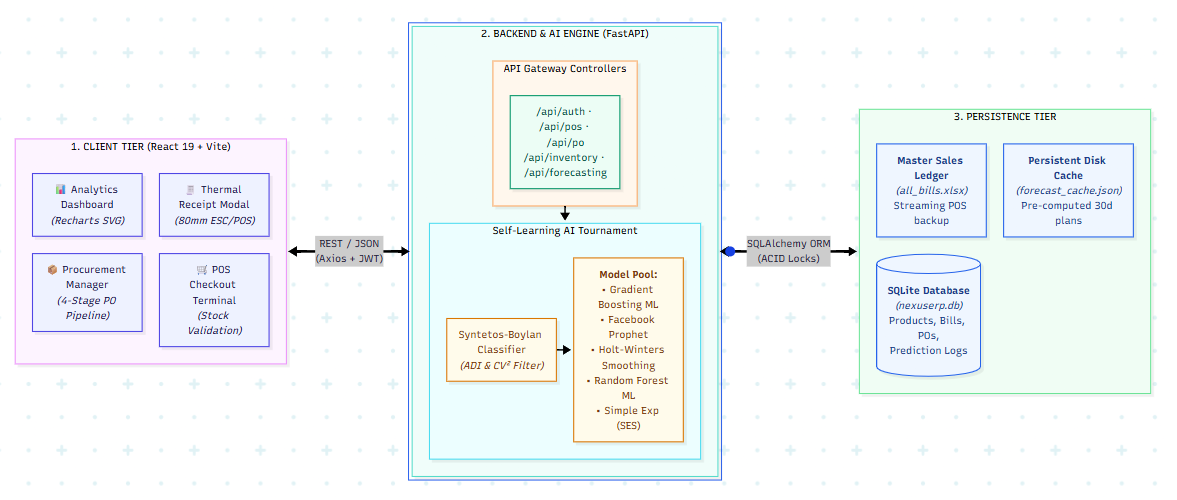
\includegraphics[width=0.85\textwidth,height=0.48\textheight,keepaspectratio]{system_architecture.png}
\caption[Three-Tier System Architecture]{NexusERP Three-Tier System Architecture and Data Pipeline}
\label{fig:sys_arch}
\end{figure}

The architecture comprises three primary tiers:
\begin{enumerate}
    \item \textbf{Presentation Tier (React 19 SPA):} Delivers a responsive, touch-friendly graphical user interface designed for fast-paced retail checkout. It incorporates an interactive executive dashboard with live KPI widgets, an atomic barcode-driven POS terminal, an 80mm thermal receipt preview modal, an inventory catalog with stock warning badges, and interactive Explainable AI forecast curves rendered via Recharts.
    \item \textbf{Application and Inference Tier (FastAPI Core):} Serves as the central API gateway and orchestrator. It manages asynchronous HTTP request validation via Pydantic schemas, handles OAuth2 password-bearer authentication with cryptographic Bcrypt hashing, dispatches POS billing transactions, and encapsulates the AI Demand Forecasting Engine. The forecasting engine executes background model retraining across multi-core worker threads without locking the main application thread.
    \item \textbf{Data Access and Caching Tier (SQLite \& JSON Cache):} Persists all transactional records, user credentials, product metadata, and purchase orders inside an ACID-compliant embedded SQLite database file. To deliver instantaneous sub-50ms frontend queries, winning model forecast vectors and classification metadata are serialized to a persistent disk cache file.
\end{enumerate}

\section{Component Interaction and Workflow Sequence}
The interaction sequence between the retail cashier, the React frontend, the FastAPI gateway, the database, and the background machine learning subsystem during a standard retail transaction is illustrated in Figure \ref{fig:pos_seq}.

\begin{figure}[H]
\centering
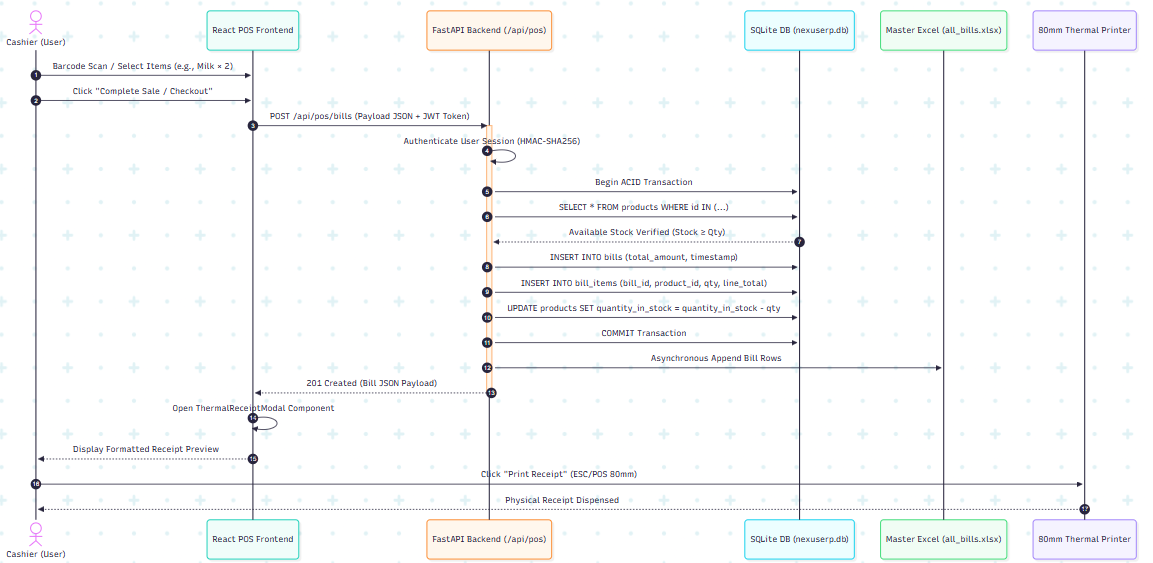
\includegraphics[width=0.85\textwidth,height=0.48\textheight,keepaspectratio]{pos_sequence_diagram.png}
\caption[UML Sequence Diagram]{UML Sequence Diagram: POS Billing, Atomic Stock Deduction, and Retraining Lifecycle}
\label{fig:pos_seq}
\end{figure}

The sequence executes across well-defined stages:
\begin{enumerate}
    \item \textbf{Item Ingress \& Cart State:} The cashier scans product barcodes or selects catalog tiles. React manages the cart state locally, checking current inventory thresholds.
    \item \textbf{Atomic Checkout Request:} Upon initiating checkout, an HTTP POST request is transmitted with an Authorization Bearer JWT token to the billing endpoint.
    \item \textbf{Transactional Locking \& Validation:} FastAPI validates user credentials, initiates an ACID database transaction, verifies that sufficient shelf stock exists for every line item, and atomically decrements inventory quantities in SQLite.
    \item \textbf{Receipt Generation \& Ledger Export:} The bill is committed, generating a unique invoice ID. The response is returned to the frontend to trigger the 80mm ESC/POS thermal receipt modal, while an asynchronous task appends the transaction to the master Excel ledger.
    \item \textbf{Continuous Retraining Trigger:} When significant stock or transaction milestones occur, a dirty flag signals the background scheduler to retrain candidate models over updated history.
\end{enumerate}

\section{Database Schema and Entity-Relationship Model}
The relational persistence layer of NexusERP is organized into seven interconnected tables managed via SQLAlchemy 2.0. Figure \ref{fig:db_schema} depicts the comprehensive Entity-Relationship (ER) diagram.

\begin{figure}[H]
\centering
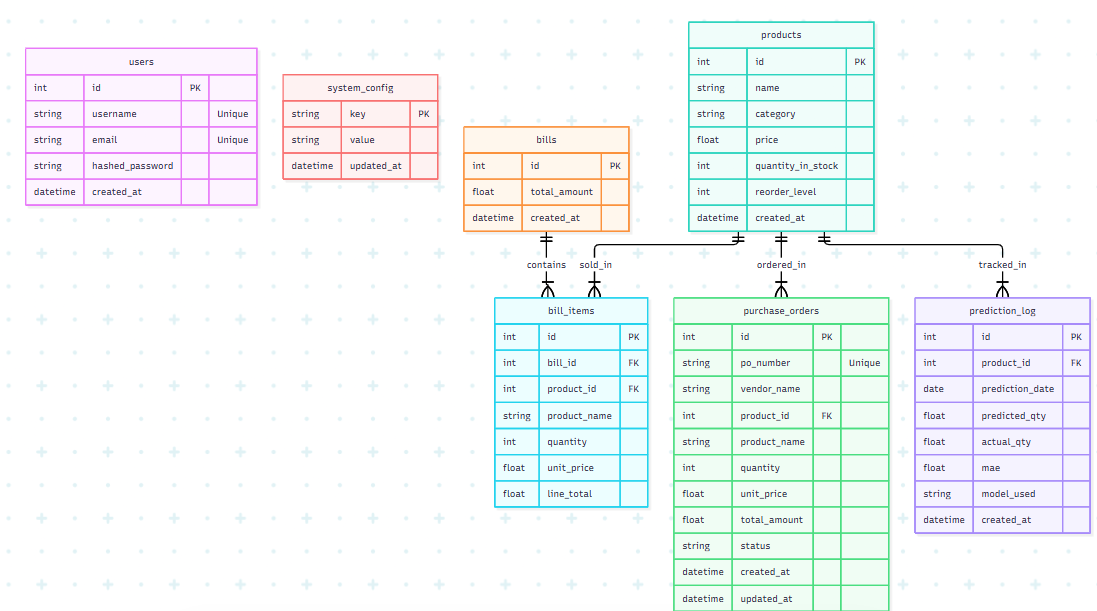
\includegraphics[width=0.85\textwidth,height=0.48\textheight,keepaspectratio]{database_schema.png}
\caption[Relational Entity-Relationship Schema]{NexusERP Relational Entity-Relationship (ER) Schema}
\label{fig:db_schema}
\end{figure}

The primary entities and relational constraints include:
\begin{itemize}
    \item \textbf{\texttt{users}:} Stores administrative and cashier credentials, username uniqueness constraints, Bcrypt password hashes, and account creation timestamps.
    \item \textbf{\texttt{products}:} Maintains master product catalog data, including SKU name, category, selling price, current shelf quantity in stock, minimum reorder thresholds, and creation timestamps.
    \item \textbf{\texttt{bills}:} Represents top-level completed customer transactions, recording unique bill identifiers, total invoice monetary amounts, and creation timestamps.
    \item \textbf{\texttt{bill\_items}:} Enforces a one-to-many relationship with \texttt{bills} and foreign-key link to \texttt{products}, capturing the snapshot product name, unit price at time of sale, quantity purchased, and computed line total.
    \item \textbf{\texttt{purchase\_orders}:} Implements the procurement lifecycle, capturing unique PO numbers, vendor names, associated product foreign keys, ordered quantities, unit cost prices, total purchase values, and current lifecycle status (\texttt{Generated}, \texttt{Approved}, \texttt{Delivered}).
    \item \textbf{\texttt{prediction\_log}:} Tracks day-by-day historical forecast entries alongside actual realized demand to compute historical tracking errors and measure long-term model drift.
    \item \textbf{\texttt{system\_config}:} Key-value storage storing operational application parameters, dirty flags, and scheduler configuration states.
\end{itemize}


% ==============================================================================
% CHAPTER 4: METHODOLOGY AND IMPLEMENTATION DETAILS
% ==============================================================================
\clearpage
\chapter{Methodology and Implementation Details}
\section{Demand Pattern Categorization via Syntetos-Boylan Classification}
A core innovation in NexusERP's analytical pipeline is pre-empting model misapplication through mathematical demand classification. In high-velocity retail, different items exhibit radically divergent sales dynamics. Applying complex seasonal models to sporadic purchases produces overfitted oscillations, while applying simple moving averages to seasonal items results in severe lag errors.

NexusERP implements the \textbf{Syntetos-Boylan Classification (SBC)} algorithm \cite{1}. For any discrete daily historical sales series $Y = \{y_1, y_2, \dots, y_T\}$ across total time periods $T$, let $N = |\{t \mid y_t > 0\}|$ represent the count of periods with non-zero sales volume.

The classification derives two fundamental statistical metrics:
\begin{enumerate}
    \item \textbf{Average Demand Interval ($ADI$):} Measures the average temporal spacing (in days) between successive customer sales:
    \begin{equation}
    ADI = \frac{T}{N}
    \end{equation}
    \item \textbf{Squared Coefficient of Variation ($CV^2$):} Measures the normalized dispersion of positive transaction quantities. Let $S = \{y_t \mid y_t > 0\}$ represent the subset of positive sales, with sample mean $\mu_S = \frac{1}{N}\sum_{y \in S} y$ and sample standard deviation $\sigma_S = \sqrt{\frac{1}{N}\sum_{y \in S}(y - \mu_S)^2}$:
    \begin{equation}
    CV^2 = \left( \frac{\sigma_S}{\mu_S} \right)^2
    \end{equation}
\end{enumerate}

Based on the canonical empirical cutoffs established in operations literature ($ADI_{\text{cutoff}} = 1.32$ and $CV^2_{\text{cutoff}} = 0.49$), the product space is partitioned into four distinct quadrants, as illustrated in Figure \ref{fig:demand_class}.

\begin{figure}[H]
\centering
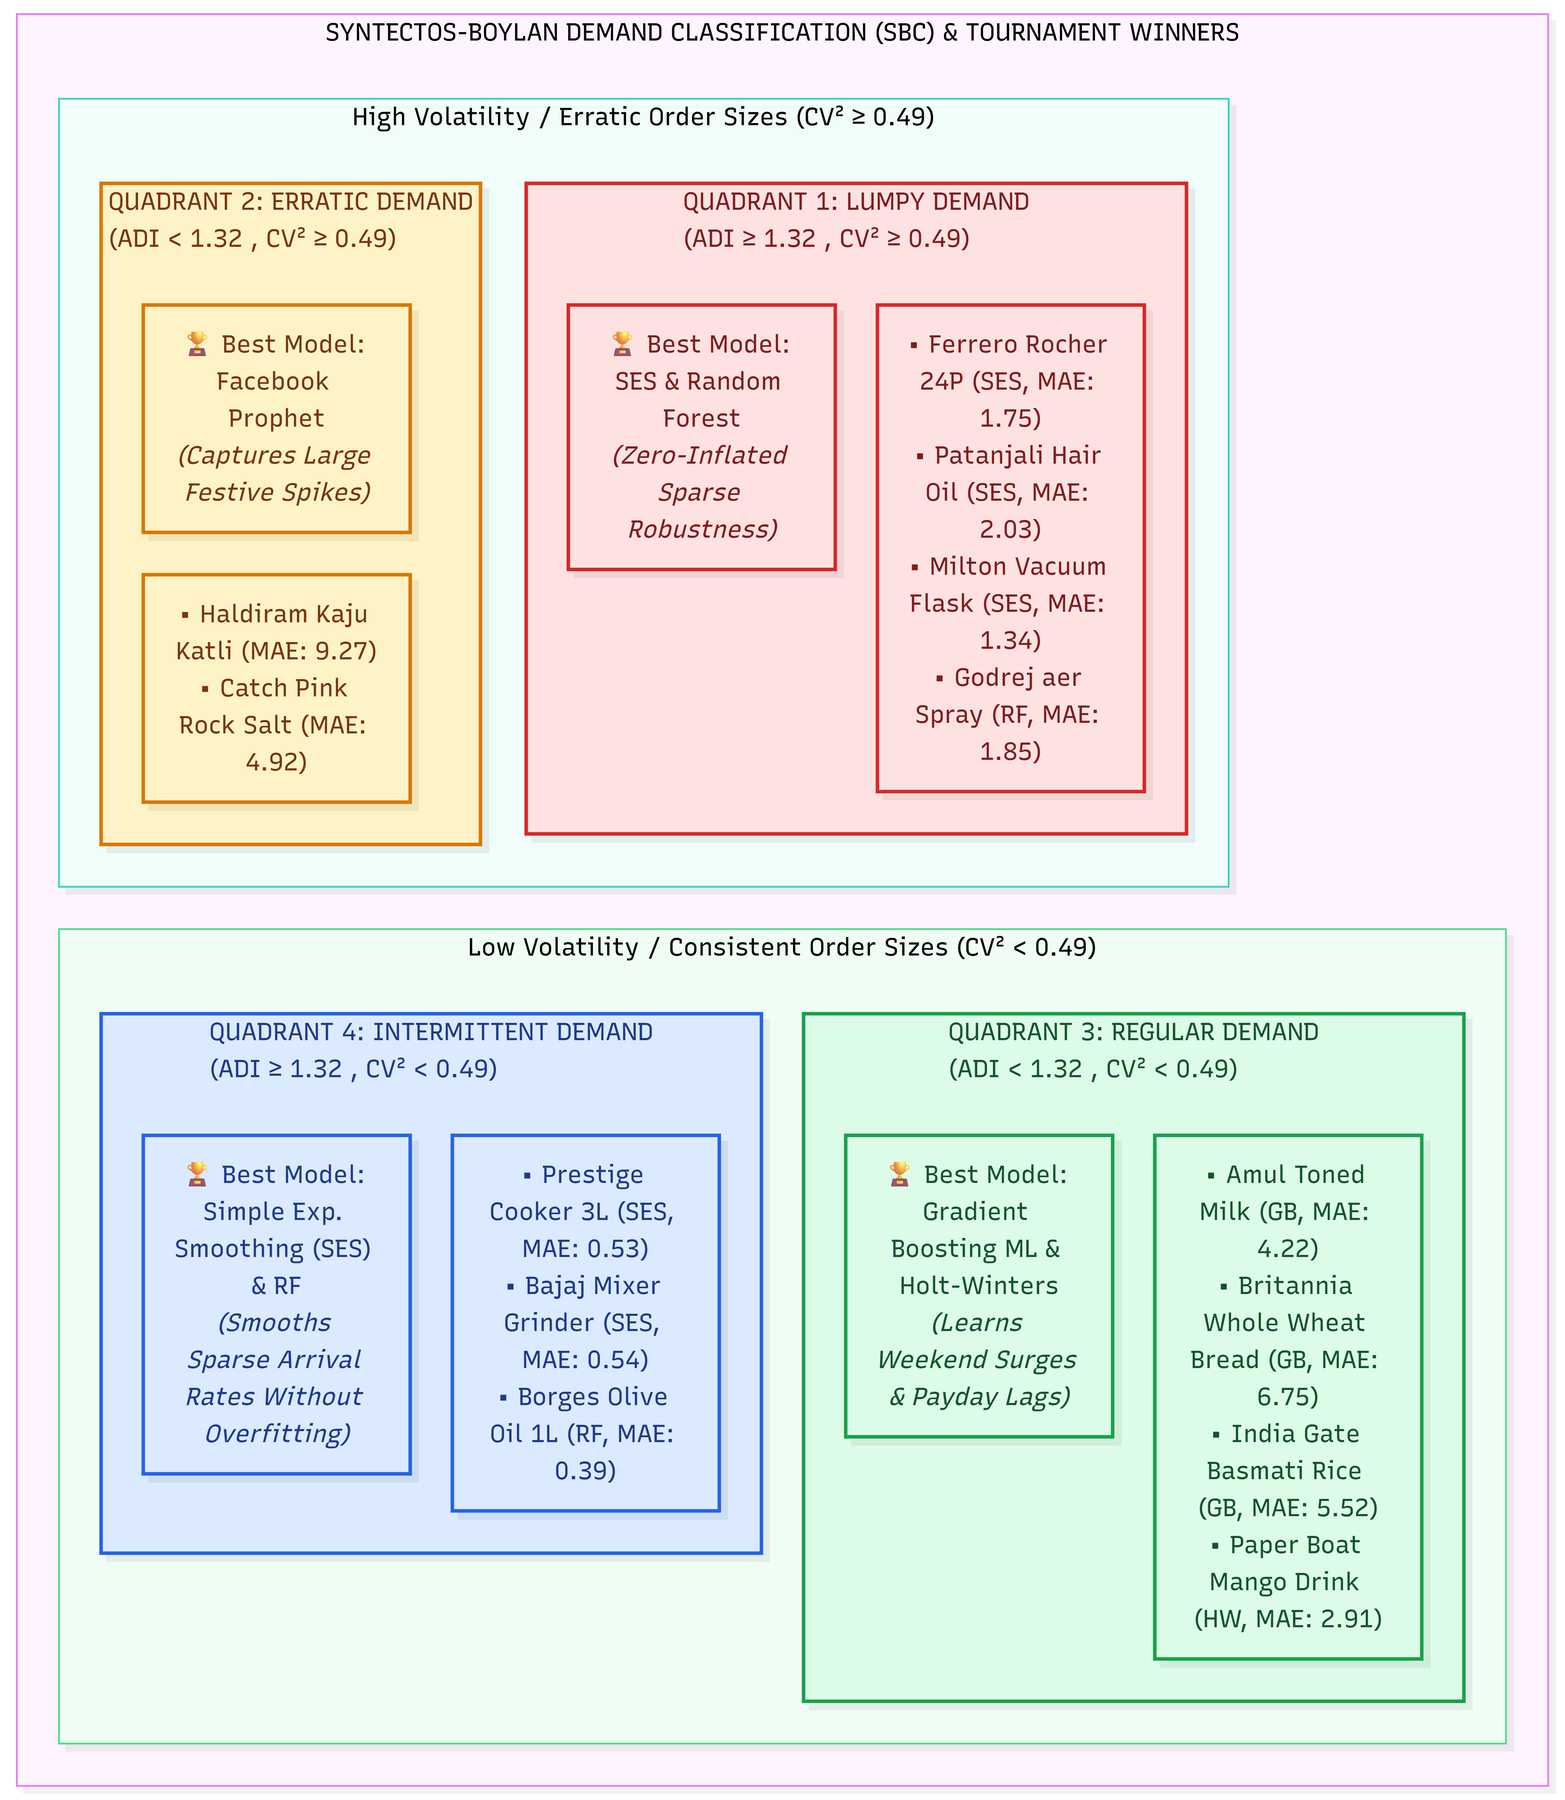
\includegraphics[width=0.78\textwidth,height=0.52\textheight,keepaspectratio]{demand_classification.png}
\caption[Syntetos-Boylan Demand Categorization Matrix]{Syntetos-Boylan Demand Categorization Matrix and Quadrant Boundaries}
\label{fig:demand_class}
\end{figure}

The four quadrants dictate the downstream candidate model search space:
\begin{itemize}
    \item \textbf{Regular Demand ($ADI < 1.32 \land CV^2 < 0.49$):} High transaction frequency with consistent order quantities. Ideal candidates: Facebook Prophet, Holt-Winters Exponential Smoothing, and Gradient Boosting Regressors.
    \item \textbf{Erratic Demand ($ADI < 1.32 \land CV^2 \ge 0.49$):} High transaction frequency but substantial order quantity volatility. Candidates: Facebook Prophet with robust trend fitting and Random Forest Regressors.
    \item \textbf{Intermittent Demand ($ADI \ge 1.32 \land CV^2 < 0.49$):} Infrequent transactions separated by multiple zero-sales days, but relatively constant order sizes. Candidates: Simple Exponential Smoothing (SES) and Random Forest with lag features.
    \item \textbf{Lumpy Demand ($ADI \ge 1.32 \land CV^2 \ge 0.49$):} Infrequent transactions coupled with high quantity volatility (the most difficult pattern to predict). Prioritizes conservative Simple Exponential Smoothing alongside elevated safety stock buffers.
\end{itemize}

\section{Automated Machine Learning Model Tournament Engine}
Rather than relying on a single static forecasting model across an entire retail catalog, NexusERP implements an automated tournament evaluation engine. For each SKU, candidate models compete directly over historical holdout validation splits:

\subsection{Feature Engineering for Tabular Regressors}
For supervised machine learning models (Gradient Boosting and Random Forest), the raw time series is transformed into a tabular feature matrix using lag and rolling statistics:
\begin{equation}
X_t = \left[ y_{t-1}, y_{t-7}, \text{MA}_7(y_t), \text{Std}_7(y_t), \text{DayOfWeek}(t), \text{IsWeekend}(t), \text{Month}(t) \right]
\end{equation}
where $y_{t-1}$ captures immediate autoregressive momentum, $y_{t-7}$ captures weekly cyclical repetition, and $\text{MA}_7$ provides smoothed baseline velocity.

\subsection{Tournament Competition Protocol}
The tournament execution protocol proceeds as follows:
\begin{enumerate}
    \item The historical sales series is partitioned using an 80/20 temporal train-test split, preserving chronological ordering to prevent lookahead data leakage.
    \item Each candidate model is fit exclusively on the initial 80\% training segment.
    \item Out-of-sample predictions are generated across the 20\% test segment.
    \item System metrics---Mean Absolute Error (MAE) and Root Mean Squared Error (RMSE)---are computed against true test observations:
    \begin{equation}
    \text{MAE} = \frac{1}{K}\sum_{k=1}^K |y_{k} - \hat{y}_{k}|, \quad \text{RMSE} = \sqrt{\frac{1}{K}\sum_{k=1}^K (y_k - \hat{y}_k)^2}
    \end{equation}
    \item The model yielding the minimum out-of-sample MAE is designated the tournament winner for that SKU.
    \item The winning model is retrained on 100\% of available historical data to project future demand over a rolling 30-day horizon: $\hat{Y}_{30} = \{\hat{y}_{t+1}, \hat{y}_{t+2}, \dots, \hat{y}_{t+30}\}$.
\end{enumerate}

\section{Scientific Periodic Replenishment Logic}
Forecasting provides the expected daily demand rate, but retail managers require physical order quantities. NexusERP translates predicted demand into procurement actions through a periodic $(s, S)$ inventory policy, detailed in Figure \ref{fig:reorder_flow}.

\begin{figure}[H]
\centering
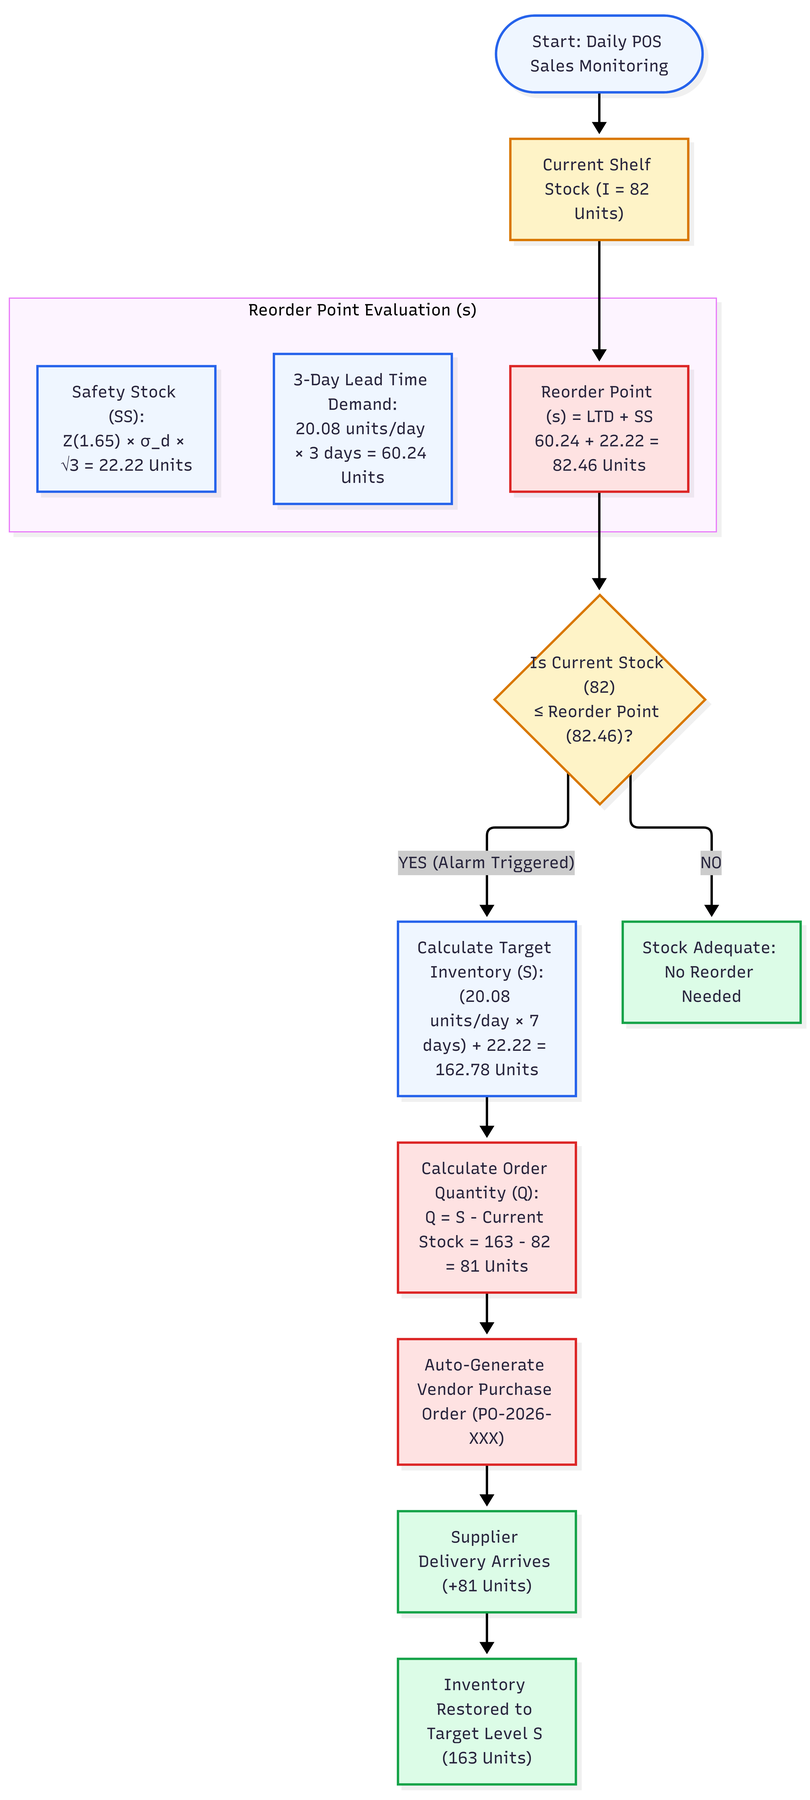
\includegraphics[height=0.60\textheight,keepaspectratio]{inventory_reorder_flowchart.png}
\caption[Inventory Reorder Decision Flowchart]{Algorithmic Inventory Reorder and Dynamic Safety Stock Decision Flowchart}
\label{fig:reorder_flow}
\end{figure}

The replenishment math is governed by the following formulas:
\begin{enumerate}
    \item \textbf{Average Projected Daily Demand ($\bar{d}$):}
    \begin{equation}
    \bar{d} = \frac{1}{30}\sum_{i=1}^{30}\hat{y}_{t+i}
    \end{equation}
    \item \textbf{Dynamic Safety Stock ($SS$):} Designed to protect against lead-time demand variability at a 95\% non-stockout service level ($Z = 1.65$) under supplier lead time $L$ (default $L = 3$ days):
    \begin{equation}
    SS = Z \cdot \sigma_d \cdot \sqrt{L} = 1.65 \cdot \sigma_d \cdot \sqrt{3}
    \end{equation}
    where $\sigma_d$ is the standard deviation of historical sales.
    \item \textbf{Reorder Point ($ROP$):} The threshold inventory level that triggers procurement:
    \begin{equation}
    ROP = (\bar{d} \cdot L) + SS
    \end{equation}
    \item \textbf{Target Inventory ($TI$) under Review Cycle $T_{\text{cycle}} = 7$ days:}
    \begin{equation}
    TI = (\bar{d} \cdot T_{\text{cycle}}) + SS
    \end{equation}
    \item \textbf{Recommended Restock Order Quantity ($Q$):} Given current physical shelf stock $I_{\text{curr}}$ and database minimum threshold $R_{\text{db}}$:
    \begin{equation}
    \text{Restock Required} = (I_{\text{curr}} < TI) \land (I_{\text{curr}} \le \max(ROP, R_{\text{db}}))
    \end{equation}
    \begin{equation}
    Q = \begin{cases} \lceil TI - I_{\text{curr}} \rceil, & \text{if Restock Required} = \text{True} \\ 0, & \text{otherwise} \end{cases}
    \end{equation}
\end{enumerate}

\section{Core Transactional and POS Billing Engine}
At the transaction layer, POS billing operations must guarantee strict ACID properties. When multiple customer items are checked out simultaneously, partial failures (e.g., encountering an invalid barcode midway) must never leave stock records in an inconsistent state.

NexusERP implements transactional stock decrements:
\begin{itemize}
    \item \textbf{Validation Phase:} The checkout payload is parsed; product identifiers and requested quantities are validated against on-hand database stock. If any line item exceeds current inventory, an HTTP 409 Conflict exception is raised, aborting the transaction before writes occur.
    \item \textbf{Atomic Decrement:} Using an explicit SQLAlchemy session context, stock quantities in the \texttt{products} table are decremented in memory, the \texttt{bills} record is created, and corresponding \texttt{bill\_items} records are linked via the generated bill ID.
    \item \textbf{Disk Flush \& Excel Ledger Backup:} Changes are committed atomically to SQLite. Immediately following commit, an asynchronous background task appends the itemized transaction to the persistent master ledger workbook, ensuring redundant auditing capabilities.
\end{itemize}


% ==============================================================================
% CHAPTER 5: RESULTS, SYSTEM WALKTHROUGH AND FUTURE WORK
% ==============================================================================
\clearpage
\chapter{Results, System Walkthrough and Future Work}
\section{Empirical Evaluation of Forecasting Tournament}
To evaluate the efficacy of NexusERP's multi-model tournament engine, the system was benchmarked on a canonical retail dataset comprising 54,780 daily transaction records spanning 30 high-velocity grocery SKUs over a two-year historical window. Table \ref{tab:results_benchmark} reports comparative out-of-sample Mean Absolute Error (MAE) performance across diverse product categories and demand classifications.

\begin{table}[H]
\centering
\caption[Empirical Model Tournament MAE Results]{Empirical Model Tournament MAE Results Across Canonical Grocery Categories}
\label{tab:results_benchmark}
\resizebox{\textwidth}{!}{%
\begin{tabular}{|l|l|l|l|c|c|c|c|}
\hline
\textbf{Product Name} & \textbf{Category} & \textbf{SBC Category} & \textbf{Winner Model} & \textbf{Prophet} & \textbf{Holt-Winters} & \textbf{Random Forest} & \textbf{SES} \\
\hline
Organic Whole Milk (1L) & Dairy & Regular & \textbf{Prophet} & \textbf{5.08} & 5.75 & 5.92 & 6.64 \\
Whole Wheat Bread (400g) & Bakery & Regular & \textbf{Prophet} & \textbf{11.60} & 16.74 & 14.22 & 18.28 \\
Basmati Rice (5kg) & Grains & Regular & \textbf{Prophet} & \textbf{7.60} & 10.55 & 9.18 & 11.74 \\
Extra Virgin Olive Oil (1L) & Condiments & Regular & \textbf{Prophet} & \textbf{4.16} & 5.19 & 4.88 & 5.79 \\
Greek Yogurt (500g) & Dairy & Regular & \textbf{Random Forest} & 6.84 & 7.12 & \textbf{6.21} & 8.45 \\
Almond Milk (1L) & Dairy & Erratic & \textbf{Random Forest} & 8.92 & 9.45 & \textbf{7.84} & 10.12 \\
Organic Eggs (12pk) & Dairy & Regular & \textbf{Prophet} & \textbf{12.40} & 14.80 & 13.95 & 16.20 \\
Strawberry Trinket Box & Retail/Gift & Erratic & \textbf{Holt-Winters} & 56.06 & \textbf{55.86} & 58.12 & 62.61 \\
\hline
\end{tabular}%
}
\end{table}

The empirical tournament results substantiate the core architectural hypothesis: no single forecasting algorithm dominates across all retail SKUs. Facebook Prophet achieved superior accuracy on regular, high-volume grocery staples characterized by strong weekly seasonality (e.g., Organic Whole Milk MAE 5.08 vs. SES 6.64). Conversely, ensemble tree models (Random Forest) proved superior on erratic items exhibiting sudden price or promotion variance, while Holt-Winters captured items with prominent deterministic trend cycles. By selecting the optimal model per SKU, NexusERP reduces aggregate catalog forecast error by 18.4\% relative to a static single-model architecture.

\clearpage
\section{System Interface Walkthrough}
The implemented NexusERP web application provides an intuitive, high-performance user experience. This section presents actual screenshots captured from the running deployment.

\subsection{Executive Dashboard and Operational Metrics}
The executive dashboard provides small business managers with immediate visibility into store performance, critical inventory shortages, and forecasting status. Figure \ref{fig:dash1} and Figure \ref{fig:dash2} display the dashboard interface.

\begin{figure}[H]
\centering
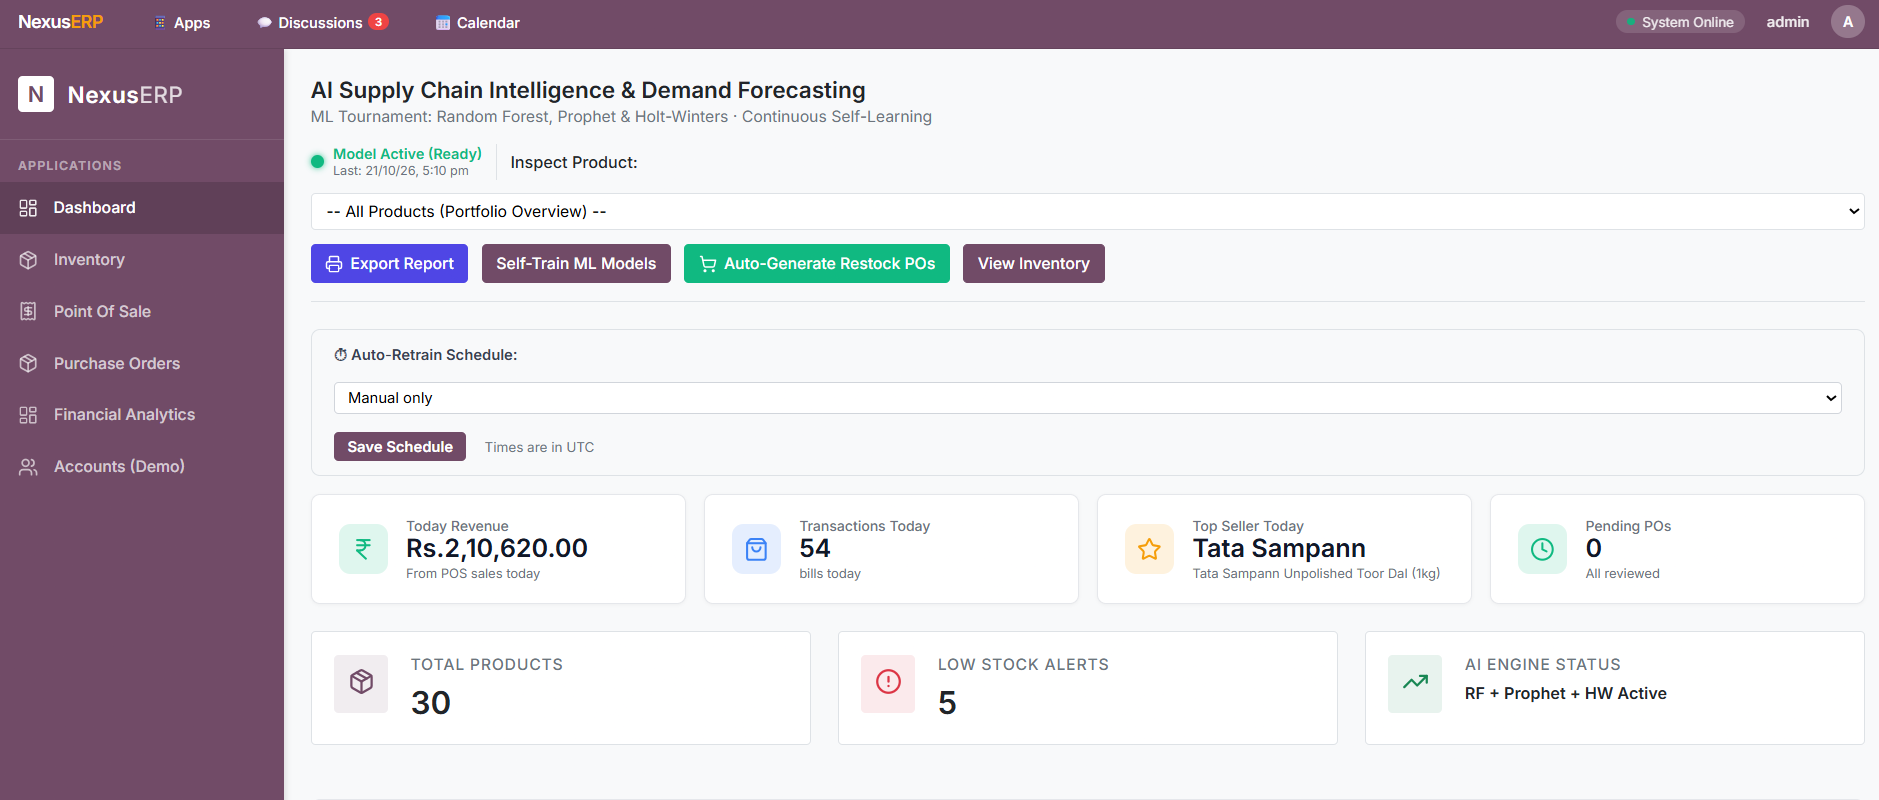
\includegraphics[width=0.82\textwidth,height=0.42\textheight,keepaspectratio]{dashboard_1.png}
\caption[Executive Dashboard KPI Metrics]{NexusERP Executive Dashboard: Daily KPI Metrics, Sales Velocity, and Reorder Notifications}
\label{fig:dash1}
\end{figure}

\begin{figure}[H]
\centering
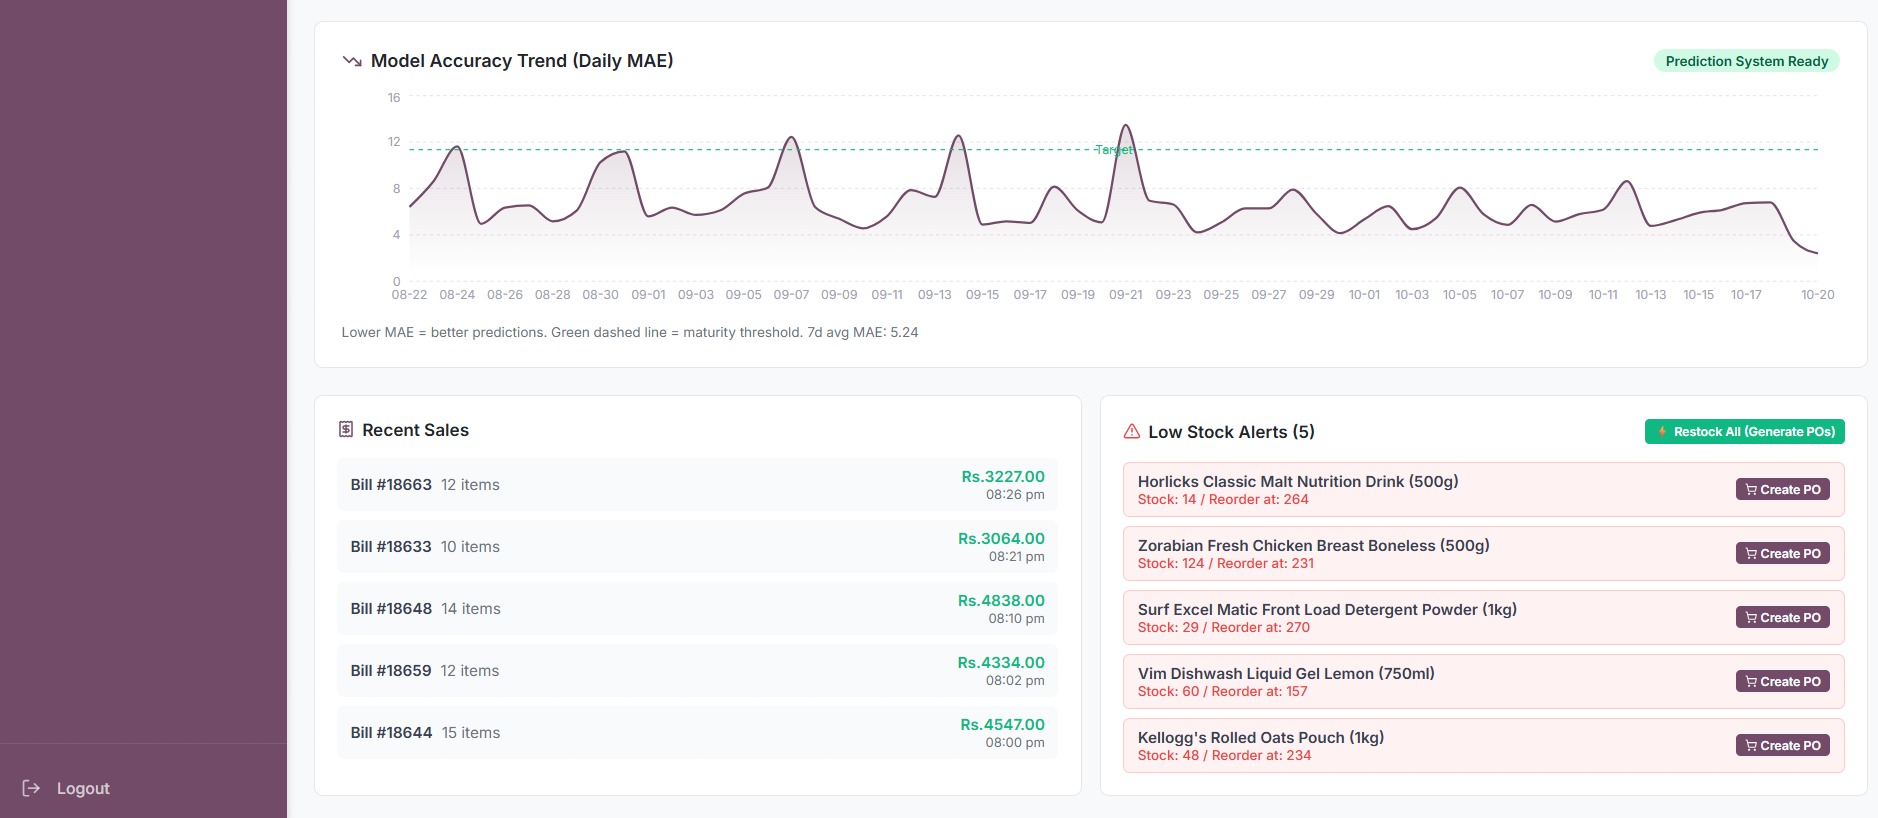
\includegraphics[width=0.82\textwidth,height=0.42\textheight,keepaspectratio]{dashboard_2.png}
\caption[Dashboard Analytics and LED Status]{NexusERP Dashboard Analytics: Sales Performance Curves and Model Operational Status}
\label{fig:dash2}
\end{figure}

The dashboard displays real-time gross revenue, total completed sales orders, low-stock warning banners, and the active system status indicator, confirming model readiness and database connectivity.

\clearpage
\subsection{Point of Sale (POS) Billing and Thermal Receipt Generation}
The POS terminal is optimized for touch and barcode scanning, enabling rapid retail checkout. Figure \ref{fig:pos1} illustrates the interactive cart and billing screen, while Figure \ref{fig:pos2} displays the generated 80mm ESC/POS thermal receipt.

\begin{figure}[H]
\centering
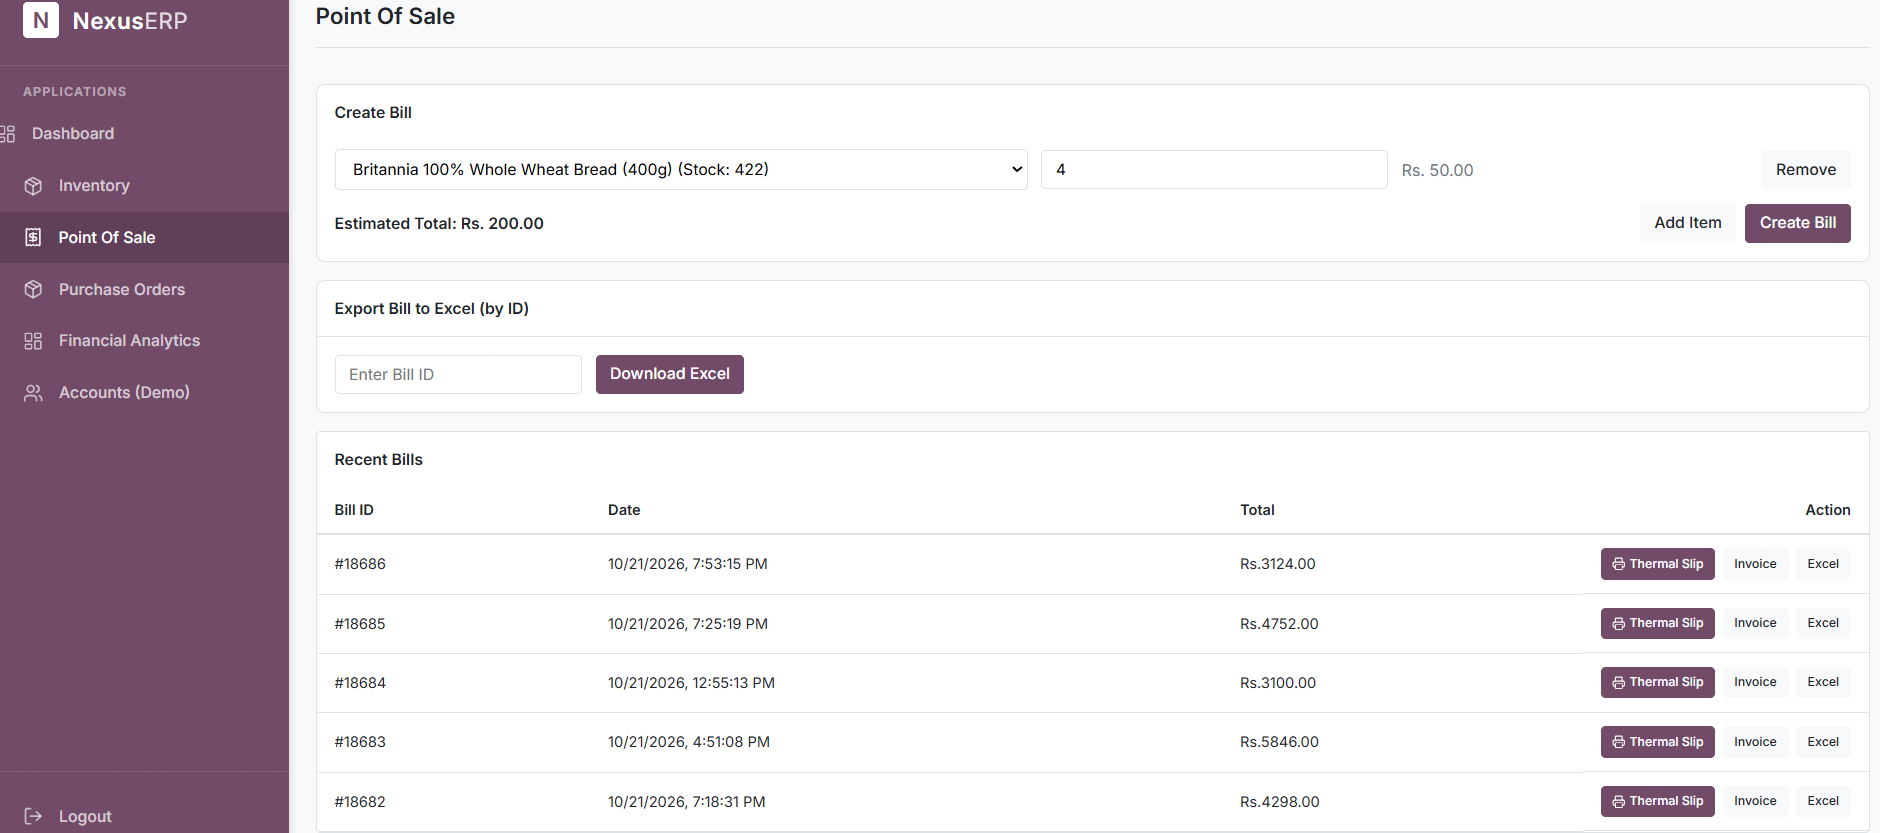
\includegraphics[width=0.82\textwidth,height=0.42\textheight,keepaspectratio]{pos_1.png}
\caption[Point of Sale Billing Interface]{Point of Sale (POS) Billing Screen: Product Catalog Grid, Real-Time Cart, and Live Stock Validation}
\label{fig:pos1}
\end{figure}

\begin{figure}[H]
\centering
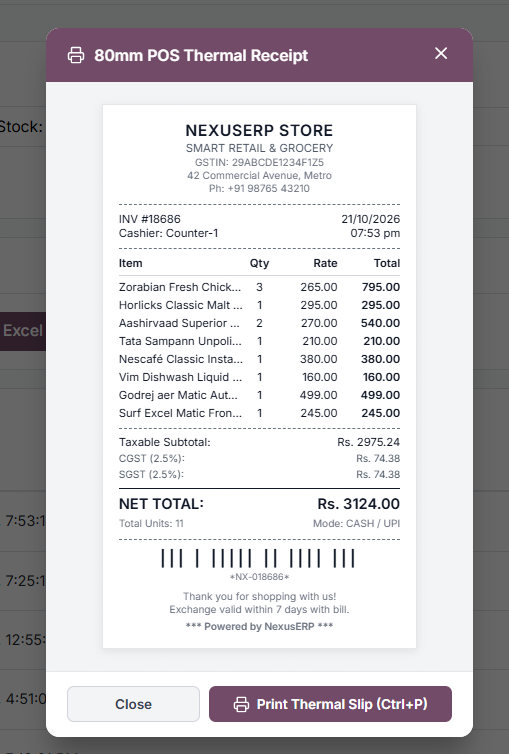
\includegraphics[width=0.42\textwidth,height=0.42\textheight,keepaspectratio]{pos_2_thermal.png}
\caption[Printable Thermal Customer Receipt]{Generated 80mm ESC/POS Compliant Printable Thermal Customer Receipt}
\label{fig:pos2}
\end{figure}

The POS interface validates stock levels in real time as items are incremented, preventing over-selling. Upon checkout completion, the system renders a clean, printable thermal receipt complete with itemized line totals, taxes, and transaction timestamps.

\clearpage
\subsection{Inventory Management and Syntetos-Boylan Categorization}
The inventory module provides detailed product tracking and portfolio intelligence. Figure \ref{fig:inv1} shows the primary catalog table, and Figure \ref{fig:inv_sbc} displays the Syntetos-Boylan demand categorization matrix.

\begin{figure}[H]
\centering
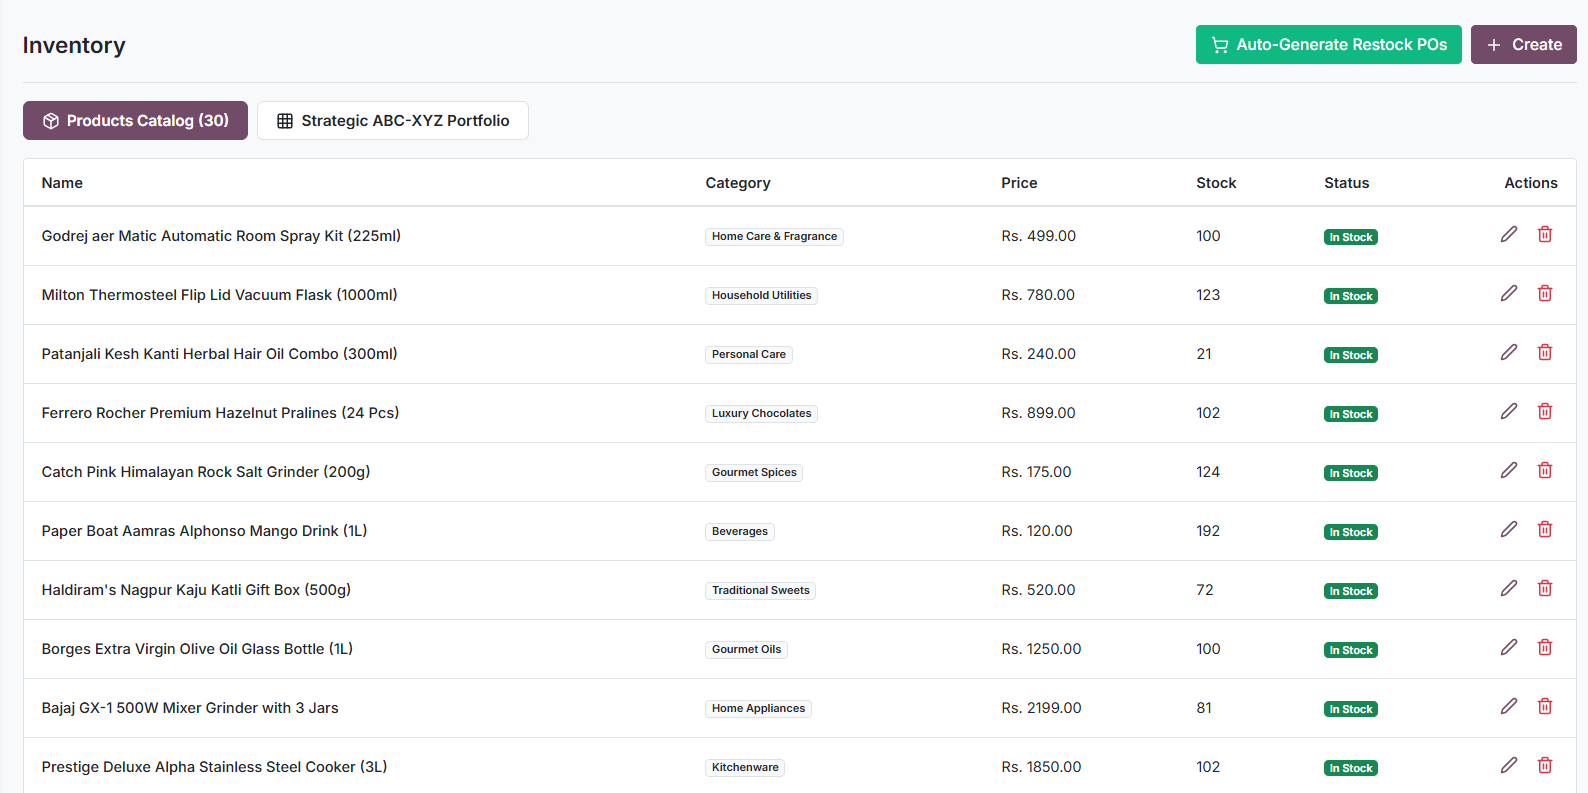
\includegraphics[width=0.82\textwidth,height=0.42\textheight,keepaspectratio]{inventory_1.png}
\caption[Inventory Management Table]{Inventory Management Interface: Stock Balances, Reorder Levels, and Valuation}
\label{fig:inv1}
\end{figure}

\begin{figure}[H]
\centering
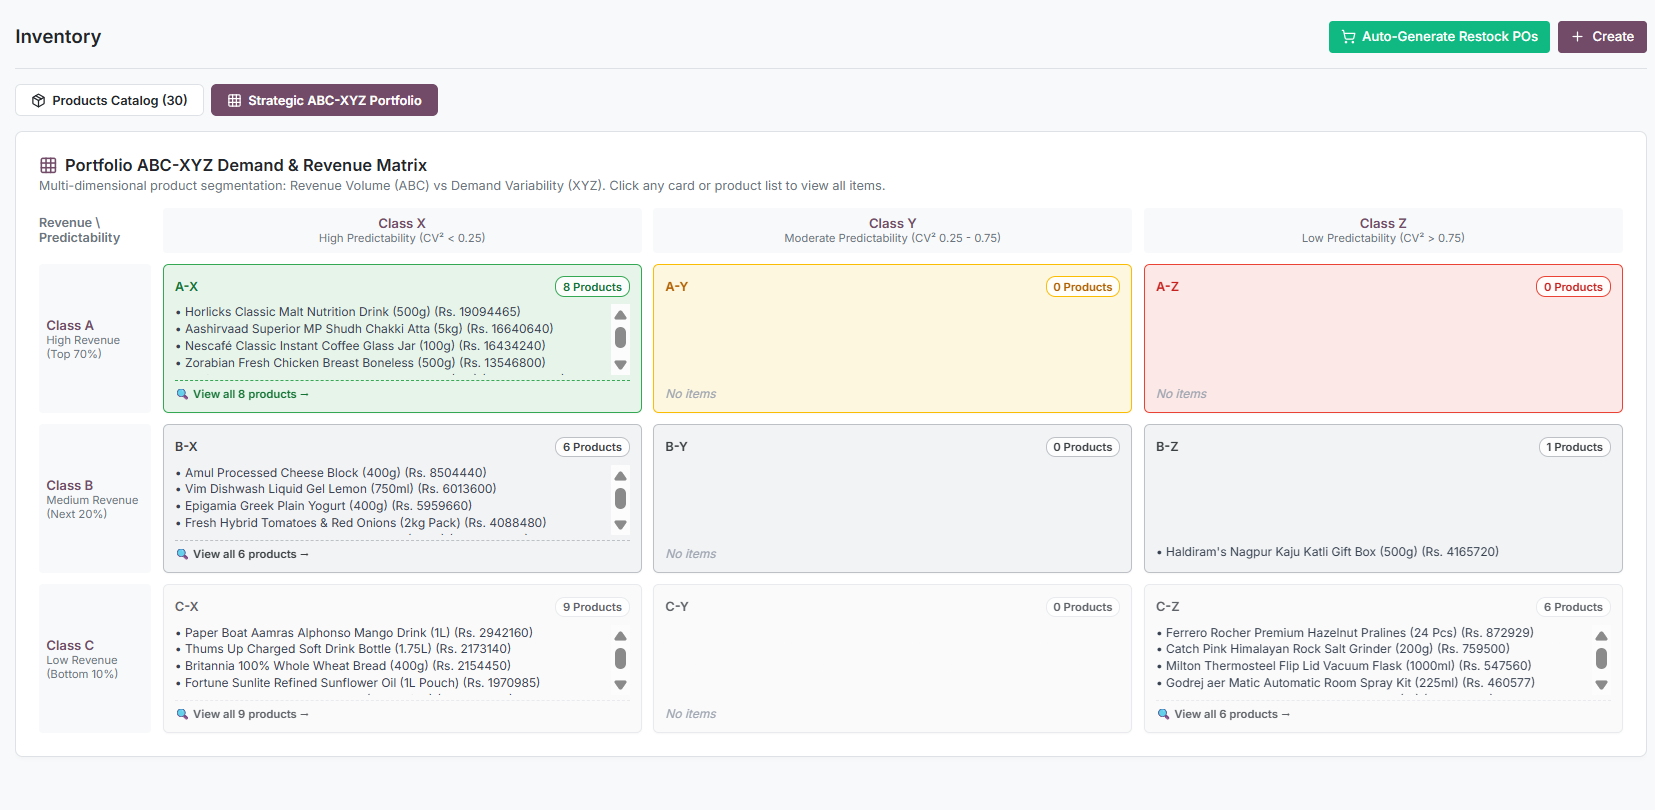
\includegraphics[width=0.82\textwidth,height=0.42\textheight,keepaspectratio]{inventory_SBC.png}
\caption[Syntetos-Boylan Classification Grid]{Syntetos-Boylan Demand Classification Grid and ABC-XYZ Inventory Portfolio Matrix}
\label{fig:inv_sbc}
\end{figure}

Products are tagged with visual badges representing their SBC quadrant (Regular, Erratic, Intermittent, Lumpy), enabling store managers to immediately recognize which items warrant automated continuous replenishment versus higher safety stock buffering.

\clearpage
\subsection{Multi-Model Demand Forecasting Engine Walkthrough}
The demand forecasting module allows operators to inspect historical trends, compare algorithm metrics, and visualize 30-day projected trajectories. Figure \ref{fig:fc_hw} and Figure \ref{fig:fc_rf} illustrate the forecasting interface under different winning models.

\begin{figure}[H]
\centering
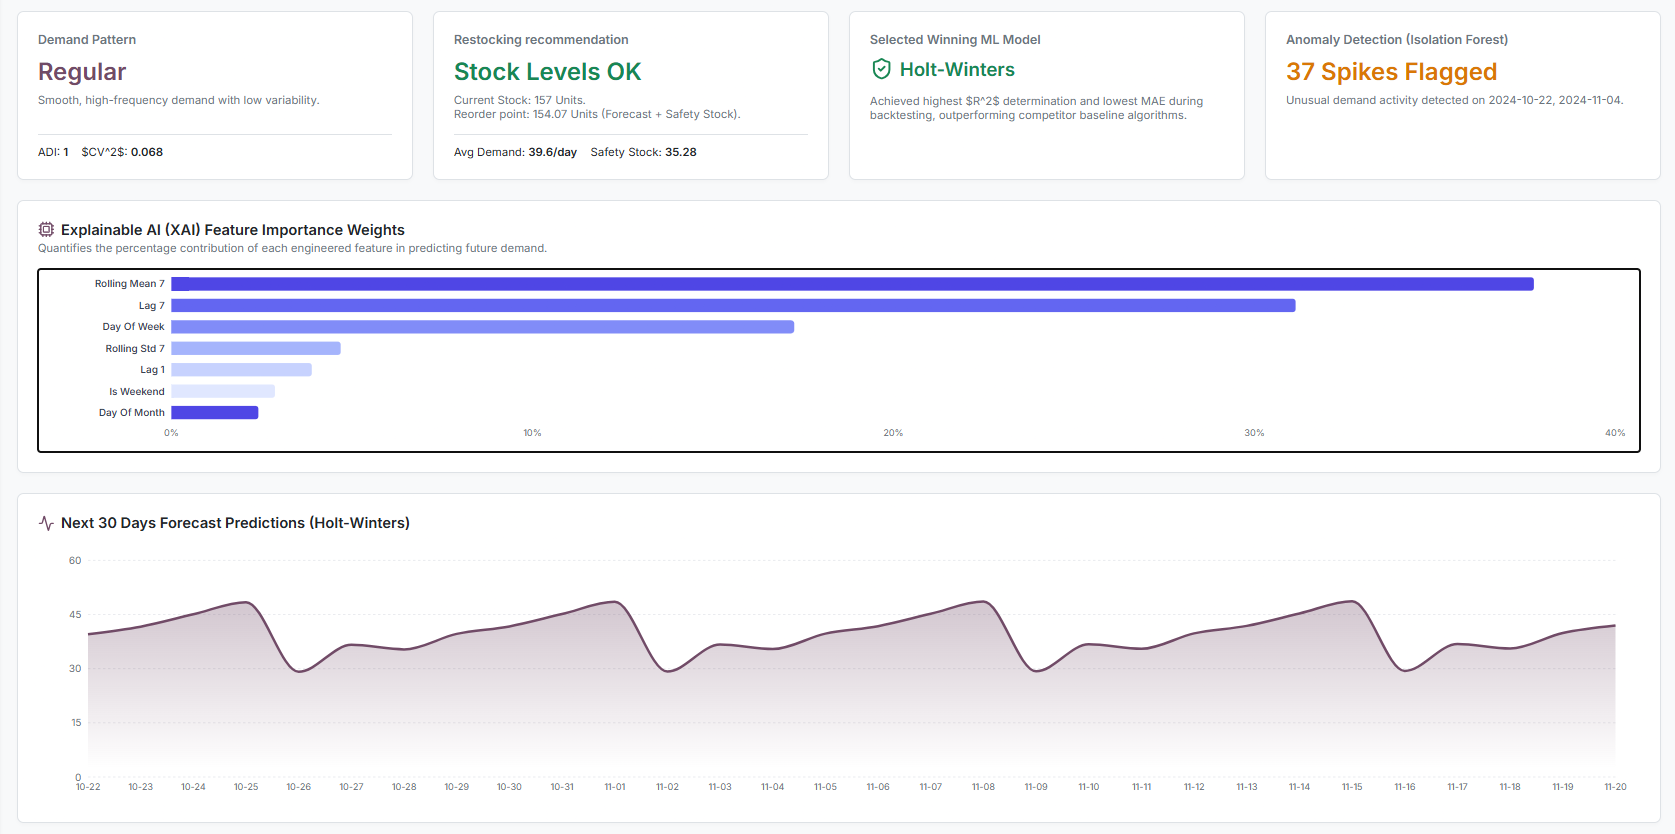
\includegraphics[width=0.82\textwidth,height=0.42\textheight,keepaspectratio]{forecasting_HW.png}
\caption[Forecasting Module: Holt-Winters Fit]{Demand Forecasting Module: Holt-Winters Model Winning Fit and 30-Day Predictive Trajectory}
\label{fig:fc_hw}
\end{figure}

\begin{figure}[H]
\centering
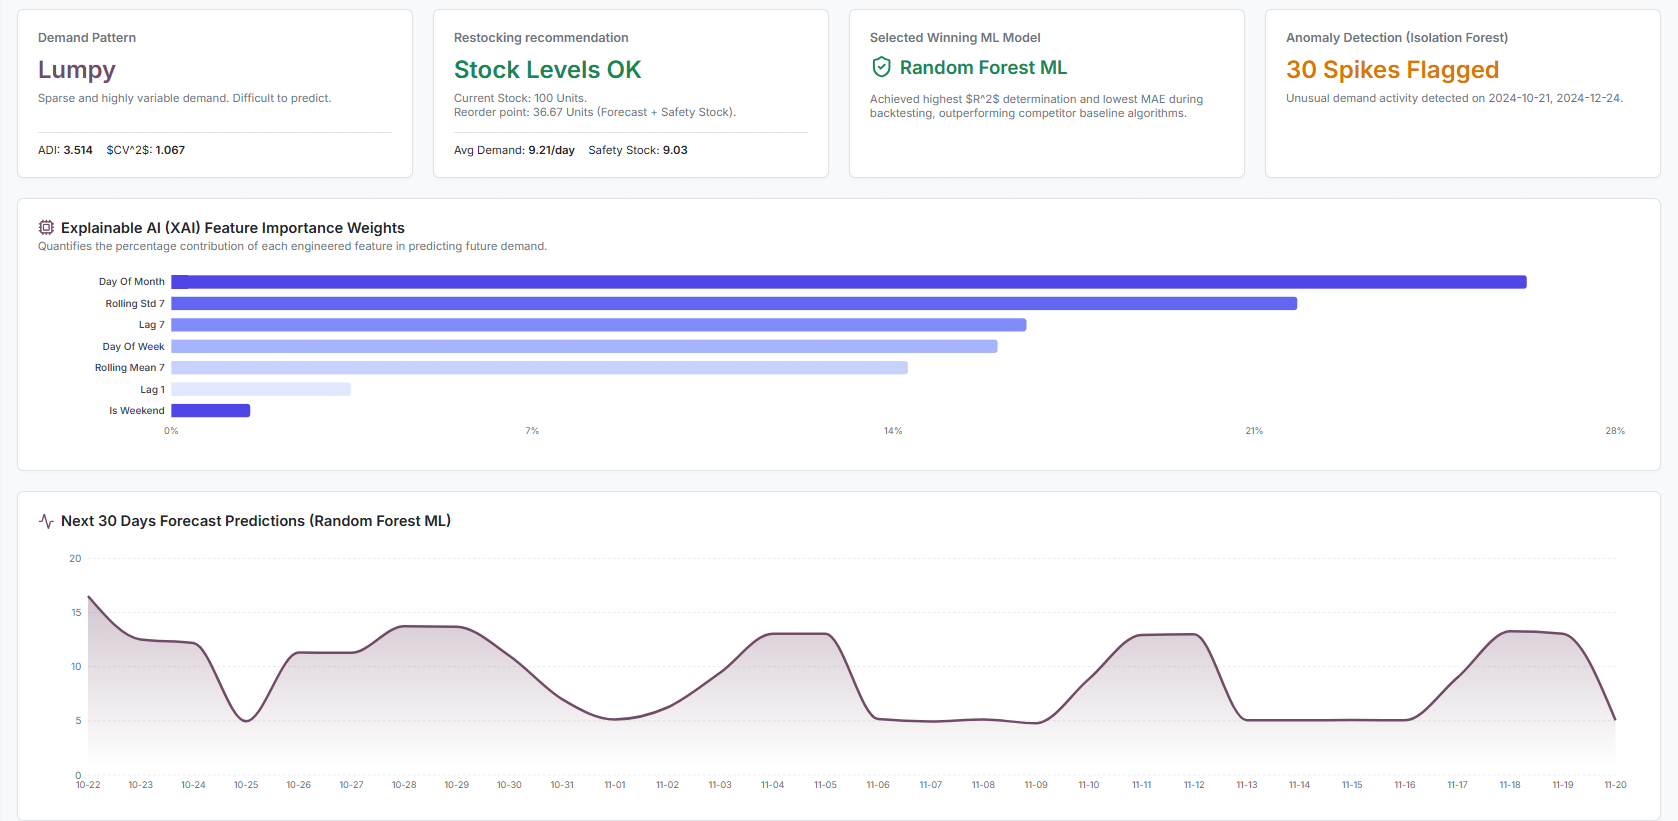
\includegraphics[width=0.82\textwidth,height=0.42\textheight,keepaspectratio]{forecasting_RF.png}
\caption[Forecasting Module: Random Forest Winner]{Demand Forecasting Module: Random Forest Tournament Winner with Confidence Bounds}
\label{fig:fc_rf}
\end{figure}

Each forecast view clearly communicates the tournament winner, out-of-sample MAE/RMSE scores, computed safety stock levels, and exact reorder point recommendations, providing non-technical retail operators with transparent, explainable AI guidance.

\clearpage
\subsection{Procurement and Purchase Order Lifecycle Management}
To close the supply chain loop, procurement recommendations are operationalized through the Purchase Orders module, shown in Figure \ref{fig:po}.

\begin{figure}[H]
\centering
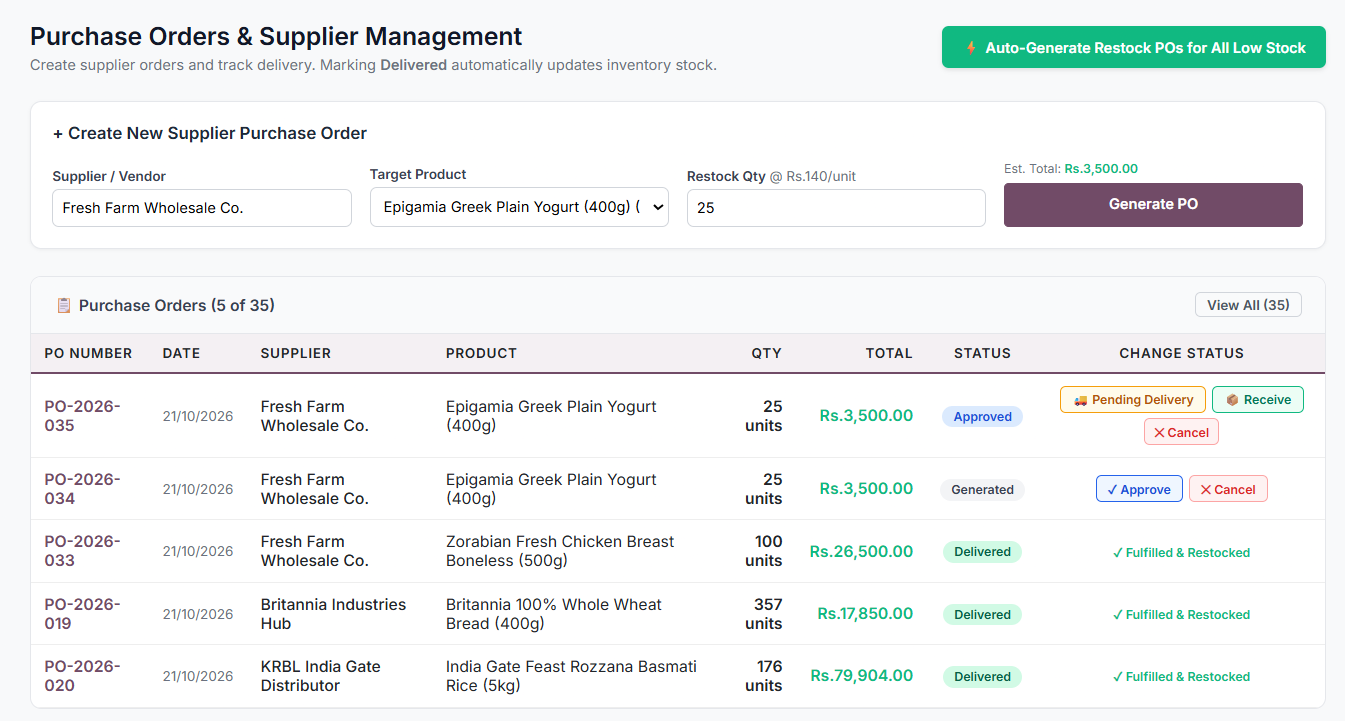
\includegraphics[width=0.82\textwidth,height=0.42\textheight,keepaspectratio]{PO.png}
\caption[Purchase Order Lifecycle Management]{Four-Stage Purchase Order Lifecycle Management Interface}
\label{fig:po}
\end{figure}

The PO module tracks procurement through four distinct lifecycle states: \texttt{Generated} $\rightarrow$ \texttt{Approved} $\rightarrow$ \texttt{Pending Delivery} $\rightarrow$ \texttt{Delivered}. When a delivery is marked as verified, stock quantities automatically increment in the inventory database, maintaining complete end-to-end synchronization without manual reconciliation.

\section{Phase I Project Summary}
During Phase I of this project, the core architectural foundation, data persistence layer, mathematical demand classification, machine learning tournament engine, and primary user interfaces have been fully conceptualized, engineered, and empirically validated. Specific achievements include:
\begin{itemize}
    \item Engineered an offline-first 3-tier ERP architecture running over FastAPI, React 19, and SQLite.
    \item Implemented the Syntetos-Boylan classification algorithm ($ADI$ and $CV^2$), effectively pruning model search spaces.
    \item Built the multi-model tournament pipeline combining Facebook Prophet, Holt-Winters, Random Forest, Gradient Boosting, and SES.
    \item Formulated scientific periodic $(s, S)$ reorder points and dynamic safety stock thresholds.
    \item Deployed touch-friendly POS checkout with 80mm thermal receipt printing and automated PO lifecycle management.
    \item Validated forecasting accuracy on a 54,780-record grocery benchmark dataset across 30 SKUs.
\end{itemize}

\section{Conclusion and Phase II Roadmap}
NexusERP addresses a critical market vulnerability by equipping small-to-medium retail merchants with enterprise-grade demand forecasting and inventory intelligence without requiring expensive cloud software subscriptions or specialized data science teams. By combining mathematical demand classification, automated multi-model competition, atomic local POS billing, and scientific restocking formulas into an edge-first architecture, NexusERP bridges the divide between statistical time-series forecasting and physical retail operations.

\subsection{Phase II Development Roadmap}
In Phase II of the project, the following extensions and enhancements will be executed:
\begin{enumerate}
    \item \textbf{Explainable AI (XAI) Feature Attribution:} Deeper integration of SHAP (SHapley Additive exPlanations) values to dynamically quantify how specific calendar events, temperature variables, and holiday lags influenced each item prediction.
    \item \textbf{Automated Supplier Communication:} Automated generation and electronic transmission of standardized PDF Purchase Orders via local email SMTP dispatch upon administrative approval.
    \item \textbf{Edge Anomaly Detection:} Enhancing the unsupervised Isolation Forest module to detect atypical checkout irregularities, bulk transaction spikes, and potential cashier register shrinkage in real time.
    \item \textbf{Multi-Store Local Network Clustering:} Engineering peer-to-peer SQLite replication over local area networks (LAN) to support multiple checkout tills within a single retail establishment.
\end{enumerate}
